\chapter[Online reprocessing simulation]{Online reprocessing simulation}

\section{Fuel salt processing systems}
\subsection{Fuel salt chemical processing facility}
All liquid-fueled \gls{MSR} designs involve varying levels of online fuel processing. Minimally, volatile gaseous fission products (e.g. Kr, Xe) escape from the fuel salt during routine reactor operation and must be captured. Additional systems might be used to intensify those elements removal rate. Most designs also call for the removal of rare earth metals from the core since these metals act as neutron poisons. Some designs suggest more complex processing elements list (figure ~\ref{fig:periodic_tab}), including the temporary removal of protactinium from the salt or other regulations of the actinide inventory in the fuel salt \cite{ahmad_neutronics_2015}.

\begin{figure}[htp!] % replace 't' with 'b' to 
  \centering
  \vspace{-0.3em}
  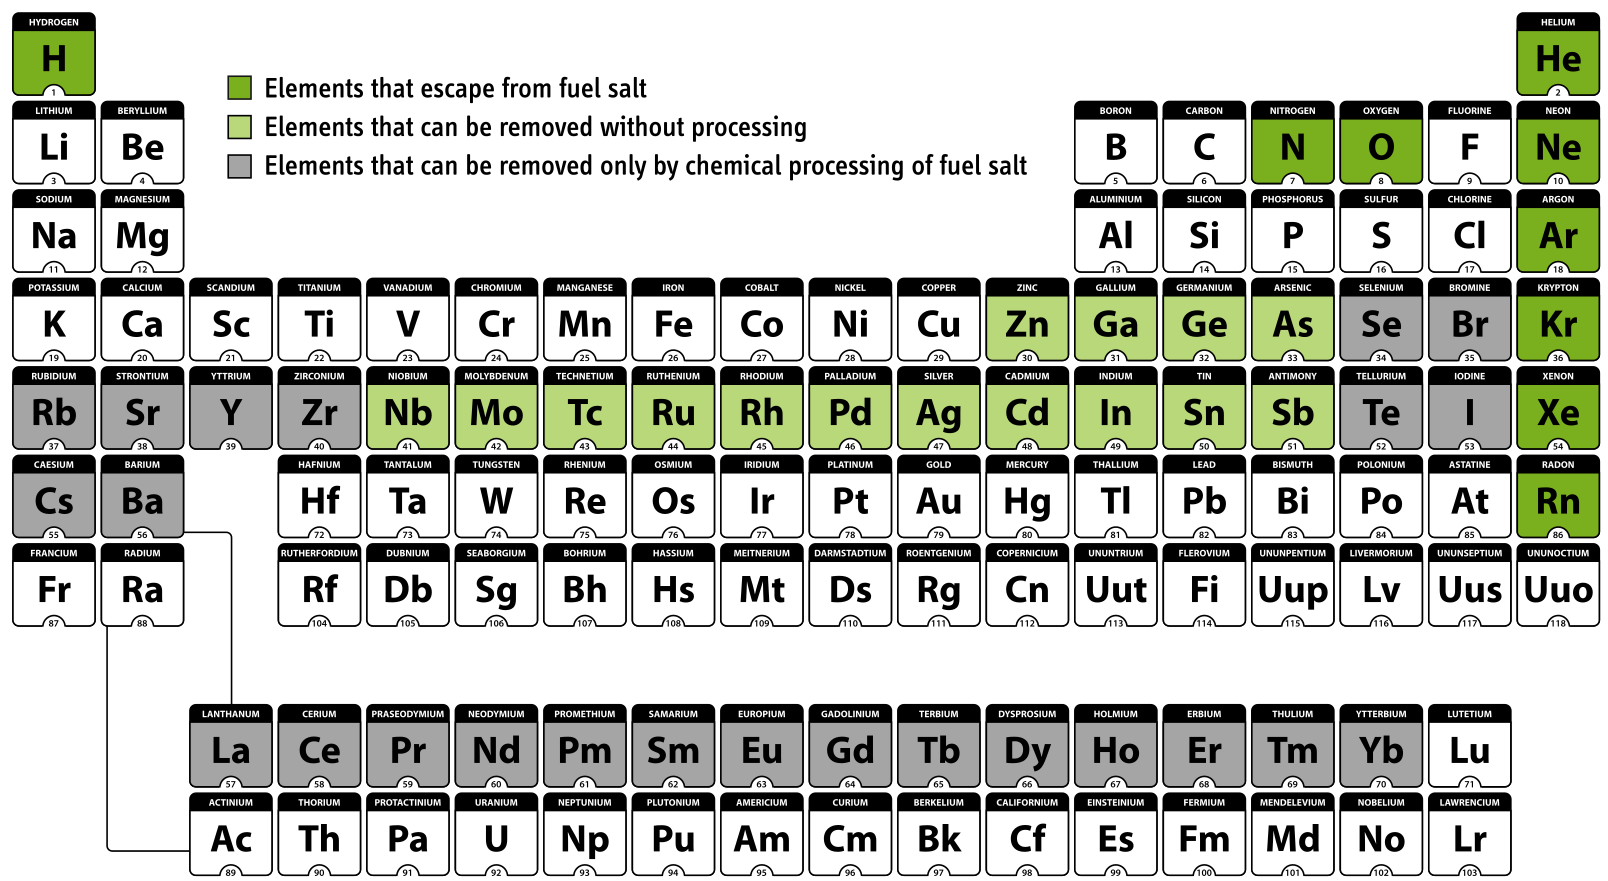
\includegraphics[width=1.05\textwidth]{periodic_map.png}
  \caption{Processing options for \gls{MSR} fuels \cite{ahmad_neutronics_2015}.}
  \vspace{-0.6em}
  \label{fig:periodic_tab}
\end{figure}
\FloatBarrier

In the one-fluid \gls{MSBR}, considered in this work, thorium, uranium, protactinium, and fission products are all mixed together in a single fluoride salt (FLiBe). Separation of thorium from lanthanide (atomic numbers 57 through 71) fission products is rather challenging because of their chemical similarities. 

Principal scheme of \gls{MSBR} reprocessing facility has shown on Figure~\ref{fig:material_flow}. Fuel salt was first held up for cooling and decay of the shortest lived fission products, then directed to the primary fluorinator, where most of the uranium was removed by fluorination to UF$_6$ using gaseous molecular form of fluorine (F$_2$) as the fluorination agent. After that the salt was routed to an extraction column where mixture containing metallic bismuth, lithium and thorium were contacted with the salt. The remaining uranium and protactinium were reductively extracted to the bismuth, leaving a salt that only contained fission products dissolved in carrier salt (base composition of LiF-BeF$_2$-ThF$_4$). This salt entered another reductive extraction column where bismuth containing lithium separated from the salt lanthanide fission products and some thorium. The salt then went through a reduction column where UF$_6$ was reduced to UF$_4$ in the salt, refueling it and preparing it for return to the reactor. Refill BeF$_2$ and ThF$_4$ were also added and all residual bismuth was removed from the salt. After a final cleanup step and valence adjustment the purified salt was returned to the reactor \cite{carter_design_1972},\cite{noauthor_one-fluid_nodate}.

The bismuth accommodating some uranium and protactinium was routed to a hydrofluorination column where the metallic solutes in the bismuth were oxidized into their fluoride forms in the presence of a decay salt. The decay salt, containing UF$_4$, PaF$_4$, and ThF$_4$ passed into a decay tank where $^{233}$Pa was decaying to $^{233}$U. This uranium generated by protactinium decay was removed through fluorination to UF$_6$ and directed to the reduction column to refuel the purified fuel salt. A hydrofluorinator and a fluorinator have capability to remove about \textbf{95\%} of the uranium from the stream.

The fully processed salt, on its way back to the reactor, has uranium added from the protactinium decay tank at the rate required to maintain or adjust the uranium concentration in the reactor (and, consequently, control the reactivity). This is performed by contacting the salt with UF$_6$ and hydrogen to produce UF$_4$ in the salt and HF gas \cite{robertson_conceptual_1971}.

\begin{figure}[htp!] % replace 't' with 'b' to 
  \centering
  \vspace{-0.3em}
  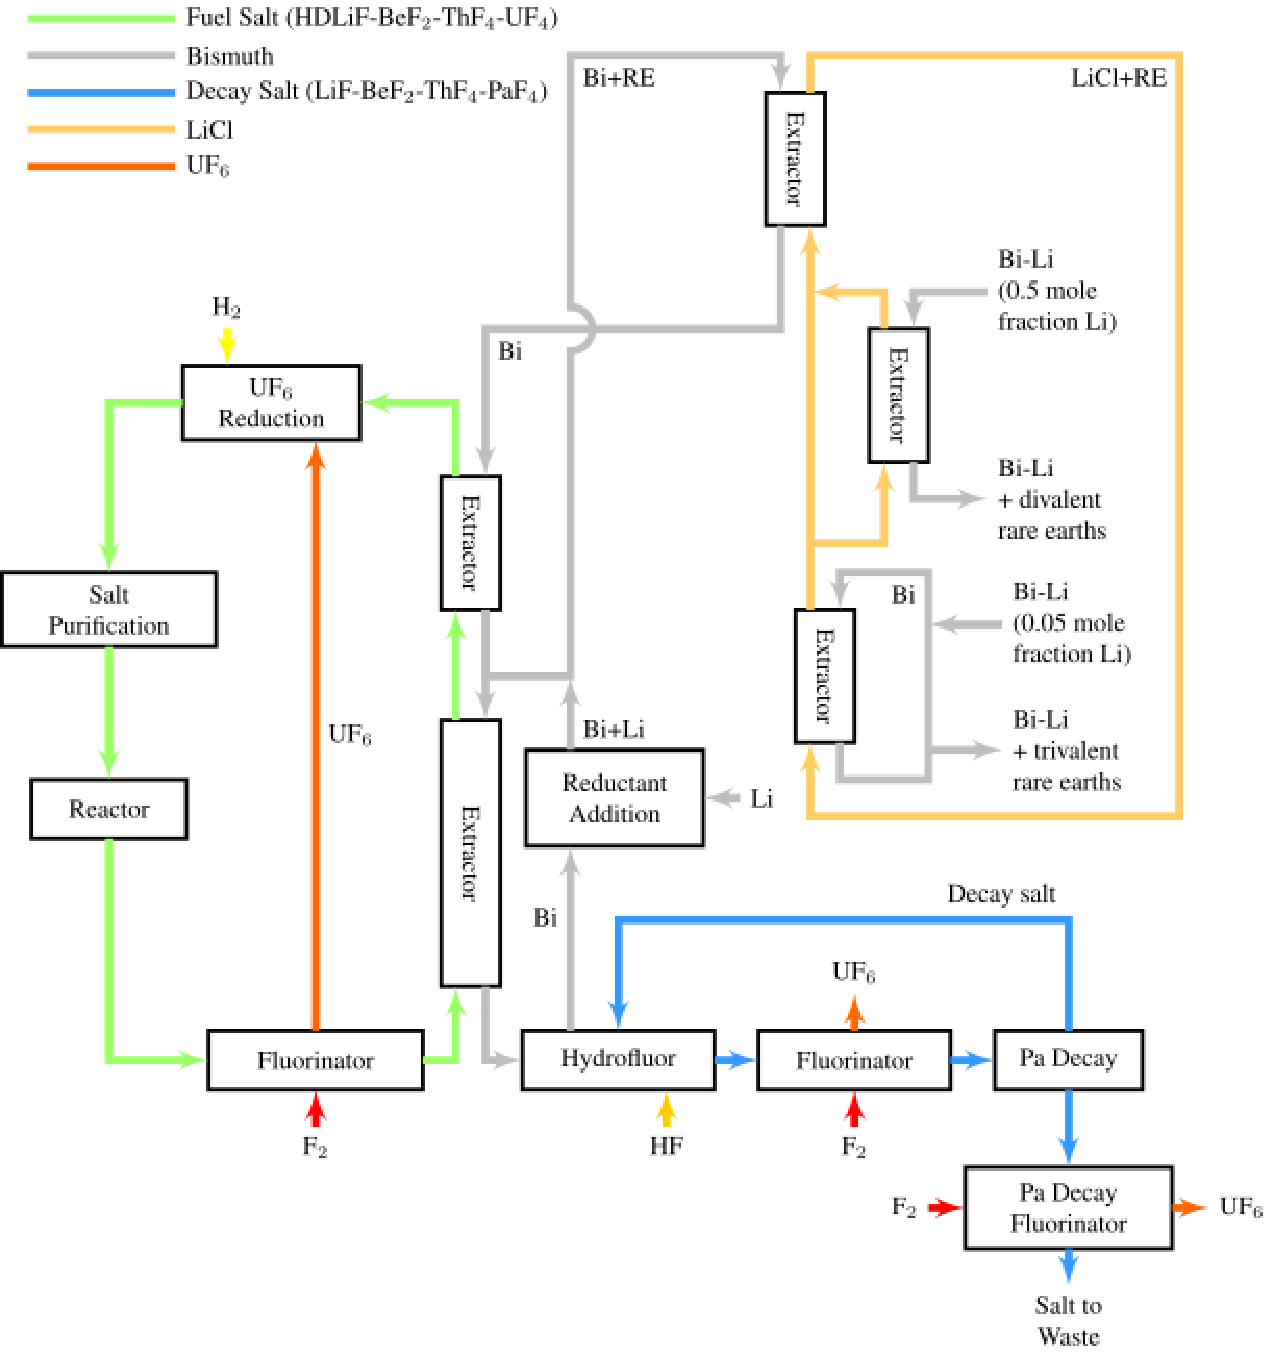
\includegraphics[width=1.05\textwidth]{flowsheet.pdf}
  \caption{Detailed block diagram of chemical processing scheme for one-fluid \gls{MSBR} \cite{robertson_conceptual_1971},\cite{noauthor_one-fluid_nodate}.}
  \vspace{-0.6em}
  \label{fig:material_flow}
\end{figure}
\FloatBarrier

\subsection{Gas separation system}
Volatile gaseous fission products (e.g. Kr, Xe) must be removed from the fuel salt to avoid reactor poisoning especially during starup and maneuvering. This is particularly true for $^{135}$Xe, with its very large absorption cross section. Tritium, xenon, and krypton are sparged from the fuel salt by helium introduced in a bypass stream by a bubble generator and subsequently removed by a gas separator. Indeed, noble gases, because of their exceptional insolubility in the salt, will migrate promptly to any gaseous interface available. Because they form a true solution in salt, they will migrate in accordance with the conventional laws of mass transfer.
If tiny helium bubbles are circulated with the fuel salt, they will absorb xenon and krypton fission products. The fission-product-rich bubbles of helium may then be separated from the salt and discharged to the off-gas system. Xenon migration to the circulating bubbles is in competition with xenon migration to the porous moderator graphite. The graphite is especially of concern because it absorbs xenon and holds it in the core which leads to parasitic neutron absorption. In \gls{ORNL} report \cite{robertson_conceptual_1971} in Appendix A it is concluded that, with moderate success of the coated-graphite program, the 0.5\% target value for $^{135}$Xe poison fraction can be achieved when circulating helium bubbles 0.508mm in diameter. This is accomplished by bypassing 10\% of the fuel salt from
the pump discharge through a bubble separator to remove the xenon bubbles, then through a clean helium bubble generator for replenishment of helium bubbles, and back into the pump suction, as shown in Figure~\ref{fig:gas_removal_system}. The average residence time of a bubble in the fuel loop would be 10 full cycles.

\begin{figure}[htp!] % replace 't' with 'b' to 
  \centering
  \vspace{-0.3em}
  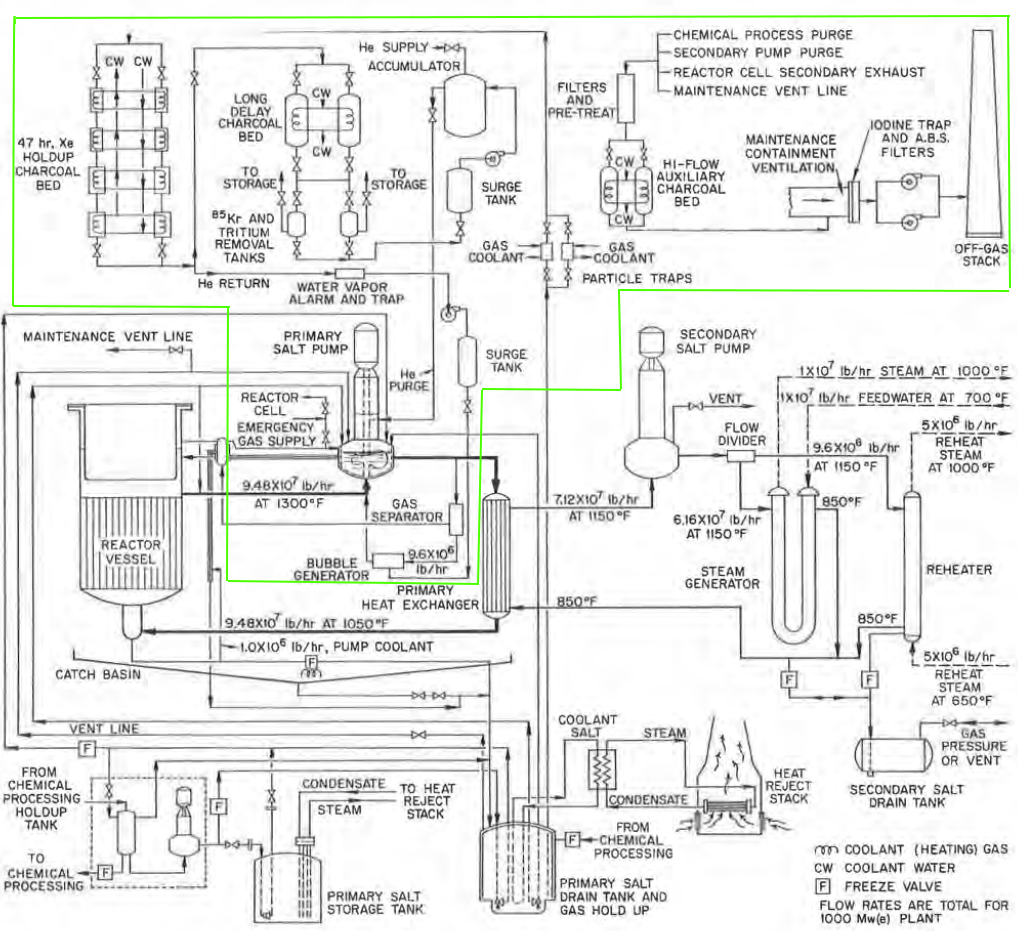
\includegraphics[width=1.05\textwidth]{gas_separation.png}
  \caption{Flow diagram for \gls{MSBR} plant. Green line indicates gas separation and off-gas system \cite{robertson_conceptual_1971}.}
  \vspace{-0.6em}
  \label{fig:gas_removal_system}
\end{figure}
\FloatBarrier
\section{Online reprocessing method}
\subsection{Online separations and feeds}
The ability to perform online reprocessing of fuel salt improves the potential neutronic performance of liquied-fueled reactors. Firstly, it is unnecessary for liquid-fueled reactors to operate with excess reactivity because fissile material is continuously adding into the core. Secondly, ability to continuously removing fission products that includes strong absorbers (poisons) might significantly improve fuel utilization and decrease neutron parasitic absorption. Finally, neutronic parameters could be adjusted ``on-the-fly" without operational cycle interruption. Nevertheless, removal of each element from the liquid fuel salt presents a exclusive problem in terms of storage and disposal of the separated materials.

To take into account online reprocessing two principal approaches might be implemented. One is a batch-wise approach where material is moved into or from the core at specific time intervals (batch). This approach based on assumption that specific material accumulation in the core during the time between separations or feeds does not affect on reactor physics. This method requires the simulation to stop at a given moment in time and restart it with a new fuel salt composition (after removal discharged materials and addition fresh fissile and/or fertile materials). This approach was implemented in a ChemTriton script \cite{powers_new_2013} which has been developed by T.J.Harrision, \gls{ORNL}, and actively using for online reprocessing simulation with SCALE/TRITON \cite{bowman_scale_2011} and Shift \cite{pandya_implementation_2016}. 

Another approach is continuous reprocessing where material is separating from (or added into) the core at all times and exactly simulate a true continuous online reprocessing. This method is more difficult because it requires adding a term to the Bateman equations. In SCALE/TRITON, ORIGEN \cite{gauld_isotopic_2011} solves a set of Bateman equations using one-group averaged fluxes and cross-sections obtained from a transport calculation. Bateman equations that describe the rate of change of the isotopes due to neutron induced reactions and decay
processes could be written in this form \cite{aufiero_extended_2013}:

\begin{align*}
\frac{dN_i}{dt}=\bar{\Phi}\sum\limits_{j}N_{j}\sigma_{j \rightarrow i} - \bar{\Phi}\sum\limits_{j}N_{i}\sigma_{i \rightarrow j} + \sum\limits_{j}N_{j}\lambda_{j}b_{j \rightarrow i} - N_{i}\lambda_{i}
\end{align*}
where $N_i,N_j$ are the number densities of isotopes $i$ and$j$;\\
$\bar{\Phi}$ is averaged in the space and energy spectrum neutron flux;\\
$\sigma_{j \rightarrow i}$ is the microscopic one-group transmutation cross section of nuclide $j$ to nuclide $i$;\\
$\lambda_i$ and $\lambda_j$ are the decay constants of nuclides $i$ and $j$;\\
$b_{j \to i}$ is the branching fraction for neutron absorption by isotope $j$ that lead to the formation of isotope $i
$.

The four terms on the right-hand side of the equation represent (1) the production rate of nuclide $i$ from irradiation, (2) the loss rate of nuclide $i$ due to irradiation, (3) the decay rate of nuclide $i$ into nuclide $j$, and (4) the loss rate of nuclide $i$ due to decay. Mentioned earlier deterministic code SCALE/TRITON and Monte Carlo codes MCNP, Shift, KENO-VI do not support non-zero removal or feeds rates for depletion simulations.

Online fuel reprocessing can be explicitly introduced in the system of equations by adding effective decay and transmutation terms for the different nuclides. During fuel composition evolution calculations, the total mass fraction of thorium fluoride is kept constant at 12\%. For this purpose, transmuted into $^{233}$Th isotope are replaced with the fresh $^{232}$Th feed material. It could be achieved by modifying the Bateman equation adding the following additional gain term to the right-hand side:
\begin{align*}
\bar{\Phi}\sum\limits_{k=^{232}Th}N_{k}\sigma_{k,c}
\end{align*}
where $\sigma_{k,c}$ is the one-group capture cross section of thorium-232.

The removal of fission products and protactinium is achieved by adding an explicit decay term to the Bateman equations. For the generic fission product l, following additonal loss term might be added:
\begin{align*}
- N_{l}\lambda_{l,reproc}
\end{align*}
where $\lambda_{l,reproc}$ is the effective removal time constant of the particular chemical specie. This approach was recently implemented as a purpose-made extension of the continuous-energy Monte Carlo reactor physics and burn-up code SERPENT \cite{aufiero_extended_2013} but it is not properly tested and unavailable for ordinary users so far.

To validate and verify in the nearest future the SERPENT 2 online reprocessing capability, I have been developed Python-based script, SaltProc \cite{andrei_rykhlevskii_arfc/saltproc:_2018}, implementing batch-wise approach on the top of SERPENT 2 burnup routine. High-fidelity full-core \gls{MSBR} model serves as a benchmark in online reprocessing simulation described in this thesis. Assessment against the SERPENT 2 continuous online reprocessing procedure based on the benchmark is not treated here.

\subsection{Fuel material flows}

The \gls{MSBR} has the capability to remove all poisons (e.g. $^{135}$Xe), noble metals, and gases (e.g. $^{75}$Se, $^{85}$Kr) every 20 seconds. The $^{232}$Th in the fuel absorbs thermal neutrons and produces $^{233}$Pa which then decays into the fissile $^{233}$U. Protactinium presents a challenge, since it has a large absorption cross section in the thermal energy spectrum. Accordingly, $^{233}$Pa is continuously removed from the fuel salt into a protactinium decay tank and allowing $^{233}$Pa to decay to $^{233}$U without poisoning the reactor. The reactor reprocessing system is designed to separate $^{233}$Pa from the molten-salt fuel over 3 days, hold it while $^{233}$Pa decays into $^{233}$U, and return it back to the primary loop. This feature allows the reactor to avoid neutron losses to protactinium, keeps fission products to a very low level, and 
increases the efficiency of $^{233}$U breeding. Table~\ref{tab:reprocessing_list} summarizes full list of nuclides and the cycle times used for modeling salt treatment and separations \cite{robertson_conceptual_1971}. 

%%%%%%%%%%%%%%%%%%%%%%%%%%%%%%%%%%%%%%%%
\begin{table}[ht!]
        \centering
        \caption{The effective cycle times for protactinium and fission product removal \cite{robertson_conceptual_1971}.}
        \begin{tabular}{|m{0.25\textwidth} | m{0.45\textwidth}|m{0.20\textwidth}|}
        \hline 
        %\begin{tabularx}{\linewidth}{l X} \toprule 
        Processing group & \qquad\qquad\qquad Nuclides & Cycle time (at full power) \\ [5pt] \hline 
        Rare earths & Y, La, Ce, Pr, Nd, Pm, Sm, Gd & 50 days \\ [5pt] \hline 
        \qquad & Eu & 500 days \\ [5pt] \hline
        Noble metals & Se, Nb, Mo, Tc, Ru, Rh, Pd, Ag, Sb, Te & 20 sec \\ [5pt] \hline
        Seminoble metals & Zr, Cd, In, Sn & 200 days \\ [5pt] \hline
        Gases & Kr, Xe & 20 sec \\ [5pt] \hline
        Volatile fluorides & Br, I & 60 days \\ [5pt] \hline
        Discard & Rb, Sr, Cs, Ba & 3435 days \\ [5pt] \hline
        Salt discard & Th, Li, Be, F & 3435 days \\ [5pt] \hline
        Protactinium & $^{233}$Pa & 3 days \\ [5pt] \hline
        Higher nuclides & $^{237}$Np, $^{242}$Pu & 16 years \\ [5pt] \hline
        \end{tabular}
        \label{tab:reprocessing_list}
          \vspace{-0.9em}
\end{table}
Since removal rates vary among nuclides in this reactor concept, the SERPENT 2 build-in reprocessing subroutine is unable to capture the desired reprocessing strategy. The removal rates also dictate the necessary resolution of depletion calculations. If the depletion time intervals are very short an enormous number of depletion steps are required to obtain the equilibrium composition. On the other hand, if the depletion  calculation time interval is too long, serious impacts of short lived fission products are not captured in a manner that is faithful \gls{MSBR} conceptual design. To compromise, the time interval for depletion calculations in this model was selected as 3 days to correlate with the removal interval of $^{233}$Pa and thorium was continuously added to maintain the initial mass fraction of $^{232}$ThF$_4$.

\subsection{Simplifying assumptions}
The main goal of present study is to identify the effects of moving materials from and to the reactor core, and find equilibrium performance of a thorium fuel cycle using \gls{MSBR}. To highlight these effects and simplify the analyses, several assumptions have been made.

First of all, thorium loading during operation was held constant and equal initial thorium loading (i.e. $m_{Th}(t)=m_0$) with variable feed rate (in kg/day) of fresh thorium. Because thorium is a fertile material with relatively high absorption cross section, this has few important impacts on reactor physics, including negatively impacting reactivity and distorting the fuel-to-moderator ratio which makes neutron energy spectrum harder. While a reduction in the thorium loading reduces the amount of initial fissile material required to achieve criticality, the breeding rate of $^{233}$U should be sufficient to maintain the core critical during operation.

The solubuluty of heavy metals is a known problem for \glspl{MSR} but it is fundamentally dependent from the type of carrier salt. For this work, solubility limits for uranium were deprioritized because the molar fraction of UF$_4$ was less than percent which considered to be reasonable to first-order for this study. In addition, it was assumed that addition or removal of soluble material (e.g. UF$_4$) has a small influence on the fuel salt volume, this volume change is not treated here.

Figure~\ref{fig:th_cycle} from Chapter 2 demonstrates that transformation $^{232}$Th to $^{233}$U takes about 30 days because $^{233}$Pa $\beta$-decay has half-life 27.4 days. Therefore, if protactinium decay tank is empty at the moment of reactor startup than expected fissile material stream would appears only after few weeks of reactor operation at full power. To avoid time-dependent feed rate for $^{233}$UF$_4$ it is assumed that protactinium decay tank contain some amount of $^{233}$UF$_4$, and the rate of fissile material flow from the tank to the core is set equal to $^{233}$Pa removal rate. Moreover, simulated cycle time at full power in this study was limited by 20 years ($\approx$ 7300 days). Finally, 100\% reprocessing separation efficiency was assumed.

The thermal fission of a $^{233}$U in fluoride salts can be shown to be an overall oxidizing process to the salt. This happens because the uranium nucleus balances the charge of four fluorine ions in the salt (e.g. $^{233}$UF$_4$), but fission products tend to not bind to all the four fluorines released after the uranium fissions. Figure~\ref{fig:excess_fluorine} demonstates an example of an oxidative fission reaction. This excess of fluorine must be compensated, otherwise chemical reactions harmful to reactor components would occur \cite{ridley_method_2017}. In this study, fission’s oxidizing effects are ignored.

\begin{figure}[htp!] % replace 't' with 'b' to 
  \centering
  \vspace{-0.3em}
  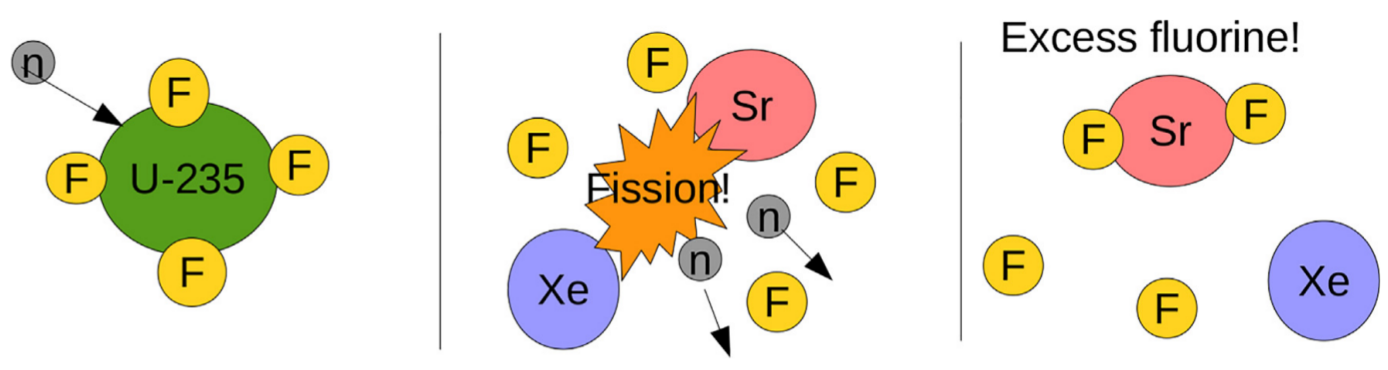
\includegraphics[width=0.8\textwidth]{excess_fluorine.png}
  \caption{Process of production an excess of fluorine due to fission of a $^{233}$U in fluoride salts \cite{ridley_method_2017}.}
  \vspace{-0.6em}
  \label{fig:excess_fluorine}
\end{figure}
\FloatBarrier

Finally, for this study equilibrium is defined as when $k_{eff}$ of the full-core model with black boundary conditions and the $^{233}$U concentration in the fuel salt are both significantly invariant in time (i.e., vary less than percent over several months). The fissile material was loaded into the system (core and protactinium decay tank) only at startup, therefore, no additional external feed or removal of fissile material assumed during reactor operation.

\section{Python code description}
The objectives for the SaltProc tool were to expand SERPENT 2 burn-up capabilities for modeling liquid-fueled \gls{MSR} and provide an open-source tool for the simulation of reactors where material is removing or adding at any time during fuel irradiation. The code written in Python 2.7, uses HDF5 \cite{the_hdf_group_hierarchical_nodate} to store data and the Nuclear Engineering Toolkit - PyNE \cite{scopatz_pyne:_2012} for SERPENT output files parsing. As was discussed earlier, SaltProc maintains the iterative semi-continuous approach to simulate a continuous feeds and removals.

The tool structure and capabilities are close to ChemTriton tool for SCALE developed in \gls{ORNL} \cite{powers_new_2013}. The primary function of SaltProc is to manage material mixtures while SERPENT 2 performs most of the computationally heavy work namely neutron transport and burnup calculations. Each material stream represents a fluid in the core design and has specific parameters (e.g. isotopic composition, reprocessing interval, mass rate, removal efficacy, etc). In addition, there is a set of available functions for each stream: read and write isotopic data in/from database, separate out specific isotopes from stream with defined efficiency, feed in specific isotopes to stream, maintain number density of specific nuclide in the core constant. These attributes and functions are crucial to simulate the operation of a complex, multi-zone, multi-fluid \gls{MSR} and are universal enough to apply it for various types of systems.

Figure~\ref{fig:saltproc_flow} demonstrates the algorithm of online reprocessing simulation with SaltProc and SERPENT 2. To perform depletion step, SaltProc reads a external SERPENT 2 template file which must be defined by user. This file contain input cards with all required for burnup calculations data such as geometry, moderator and construction materials isotopic composition, neutron population, criticality cycles, total heating power, boundary conditions. After depletion calculation completes, SaltProc reads the burned fuel composition file into memory and store it into HDF5 database. SaltProc only knows the number density and isotopic composition of a given fuel stream which provides the tool with the flexibility to model any geometry: an infinite medium, a unit cell, a multi-zone simplified assembly, or a full-core. While in some applications the simple sigle-cell is sifficient to get an accurate results within the fuel for depletion calculations with reduced simulation time, this flexibility provides high-fidelity full-core geometry capabilities for comparisons to more scrupulous models.

\begin{figure}[htp!] % replace 't' with 'b' to 
  \centering
  \vspace{-0.3em}
  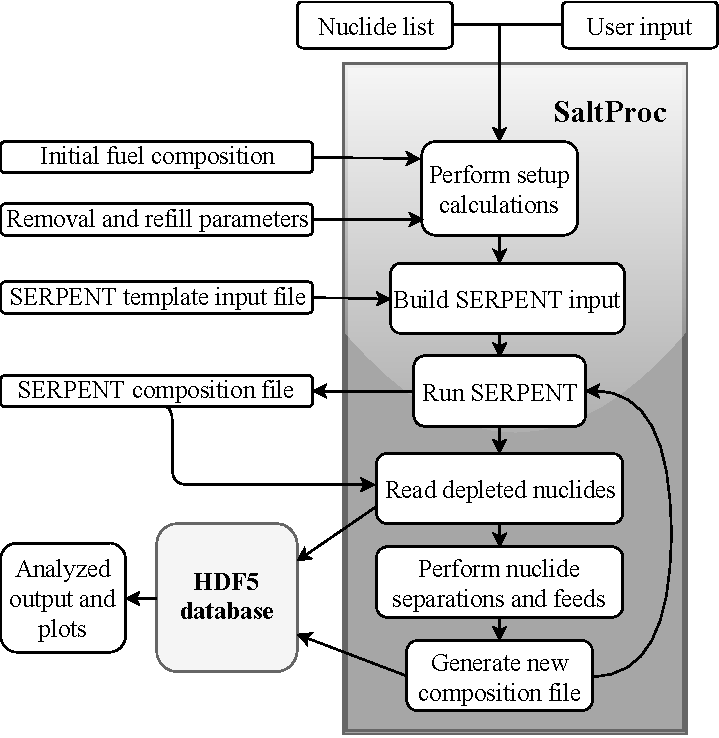
\includegraphics[width=\textwidth]{saltproc_flowchart.pdf}
  \caption{Flow chart for the Saltproc python-based tools.}
  \vspace{-0.6em}
  \label{fig:saltproc_flow}
\end{figure}
\FloatBarrier

SaltProc could manage as many fuel streams as desired. It also may work with multiple depletion materials. At the end of a each depletion step, SaltProc reads the separate depleted compositions and tracks each material stream individually. Following this, chemical reprocessing functions applying to fuel stream vectors. These vectors then combining in matrix, storing in database and printing into SERPENT composition file for the next step calculations.

Liquid-fueled \gls{MSBR} design focuses on the state of the core at an equilibrium condition, after fission products have built up in the fuel salt during years if operation. Changes in isotopic composition of the fuel salt continues encounter small changes even after decades of operation, but the dominant nuclides that have significant impact to the neutronics behavior tend to reach an equilibrium concentration (e.g., vary less than 1\% over several years). In contrast, from the startup of an \gls{MSBR} until equilibrium condition, the fuel salt composition undergo significant changes (e.g., fission producs, minor actinides, and fissile materials number density). During this period, the material feeds and removals should be optimized for the fastest \gls{MSBR} transition to an equilibrium state, where the material streams are more constant in time. A faster transition simplifies the reactor operation because in an equilibrium state the fissile and fertile feed rates, safety parameters, and fission product removal rates are more constant in time.

In addition, SaltProc is able to define time-dependent material feed and removal rates to investigate the effect of different nuclide separations and/or feeds. The time dependence of the streams could be define as piecewise functions and could be dependent on certain conditions being met. For instance, the tool could increase fissile material feeding rate if effective multiplication factor, $k_{eff}$, below a specific limit. Moreover, it could be useful to keep fissile material number density in the core approximately constant to accumulated excess of $^{233}$U into protactinium decay tank. These capabilities allow SaltProc to investigate the effect of lower concentrations of fissile and fertile startup loads. In sum, the development approach of SaltProc focused on producing a generic and flexible tool to give SERPENT 2 Monte Carlo code the ability to conduct advanced fuel cycle analysis as well as simulate a myriad of online refueled systems.
